% Standalone figure for R2.2 (blade size).
% Uses a downscaled copy of the manuscript's deposit render for a
% lighter letter PDF; colorbar is shared with the manuscript figure.
%
% Compile: pdflatex fig_r2_2.tex
\documentclass[border=5pt]{standalone}
\usepackage{tikz}
\usetikzlibrary{arrows.meta, calc}
\usepackage{amsmath}
\usepackage{siunitx}
\usepackage{graphicx}
% Local (downscaled) deposit PNG, then the shared manuscript figures/.
\graphicspath{{../shared/}{../../../../figures/}}

\begin{document}
\begin{tikzpicture}
  \node[anchor=north west, inner sep=0] (imgA) at (0,0)
    {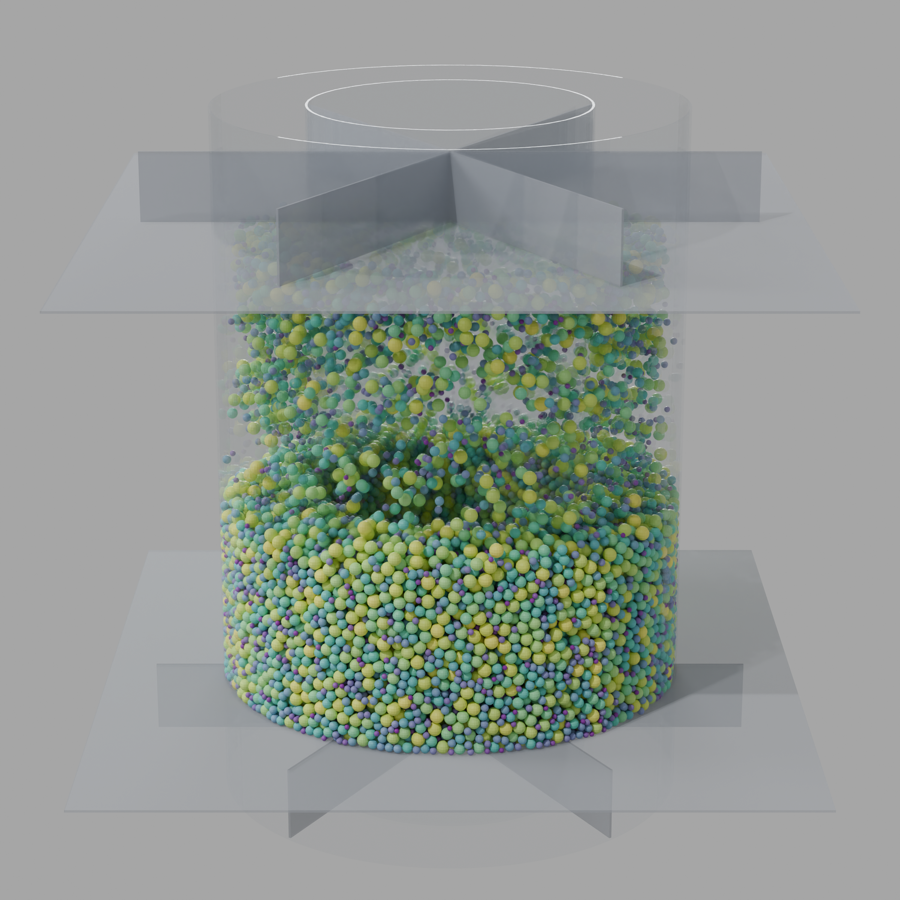
\includegraphics[height=6cm]{specimen_generation_deposit_small.png}};
  % --- h_b (blade height) dimension, normalized image coords (0,0)=SW ---
  \begin{scope}[
    x={($(imgA.south east)-(imgA.south west)$)},
    y={($(imgA.north west)-(imgA.south west)$)},
    shift={(imgA.south west)},
  ]
    \draw[{Stealth[length=3pt]}-{Stealth[length=3pt]}, thin, black]
      (0.152, 0.83) -- (0.152, 0.75);
    \node[font=\footnotesize, anchor=east] at (0.152, 0.768)
      {$h_b$};
  \end{scope}
  % --- Colorbar (shared with manuscript Fig. 1) ---
  \node[anchor=north west, inner sep=0] (cbar)
    at ([xshift=6pt]imgA.north east)
    {
\includegraphics[height=6cm]{colorbar_viridis.png}};
  \foreach \val/\frac in {1.5/0, 1.25/0.25, 1.0/0.5, 0.75/0.75, 0.5/1.0} {
    \node[font=\footnotesize, anchor=west] at
      ([xshift=2pt, yshift={-\frac*6cm}]cbar.north east) {\val};
  }
  \node[font=\footnotesize, rotate=90, anchor=south] at
    ([xshift=40pt]cbar.east) {Particle radius (mm)};
\end{tikzpicture}
\end{document}
